\section{Mạng cộng tác đồ thị chú ý (CGAT)}
Trong phần này chúng tôi mô tả lại bài toán nhúng đồ thị (Graph Embedding), sơ lược về các kỹ thuật nhúng đồ thị hiện tại. Cùng với đó chúng tôi sẽ trình bày phương pháp GAT (Graph Attention Network) và phương pháp KBGAT (Knowledge Base Graph Attention Network) mà chúng tôi đã nghiên cứu.
% Cuối cùng chúng tôi đưa ra đề xuất của chúng tôi dựa trên các mô hình trên bằng cách cộng tác thay vì ghép các lớp chú ý lại với nhau.

\subsection{Nhúng đồ thị(Graph Embedding)}
Đồ thị là một biểu diễn dữ liệu quan trọng xuất hiện trong nhiều tình huống thực tế. Khai thác đồ thị hiệu quả cung cấp cho người dùng hiểu sâu hơn về những gì đằng sau dữ liệu và do đó có thể mang lại lợi ích cho nhiều ứng dụng hữu ích như phân loại node(node classification), đề xuất node(node recommendation), dự đoán liên kết(link prediction), v.v. . Nhúng đồ thị là một cách hiệu quả để giải quyết vấn đề khai thác, phân tích đồ thị. Cụ thể, nhúng đồ thị là khái niệm biến đổi đồ thị vào không gian khác có số chiều thấp trong đó thông tin của đồ thị được lưu giữ. Bằng cách biểu diễn một đồ thị dưới dạng một hoặc một tập hợp vectơ có số chiều thấp, để các thuật toán đồ thị sau đó có thể được tính toán một cách hiệu quả.

Nhúng đồ thị vào không gian chiều thấp không phải là một nhiệm vụ tầm thường. Những thách thức của việc nhúng đồ thị phụ thuộc rất nhiều vào cách cài đặt của bài toán (problem setting), bao gồm đầu vào nhúng và đầu ra nhúng. Chúng tôi chia đồ thị đầu vào thành bốn loại như được chia ra trong khảo sát \cite{cai2018comprehensive}, bao gồm đồ thị đồng nhất(homogeneous graph),đồ thị không đồng nhất(heterogeneous graph), đồ thị với thông tin phụ trợ và biểu đồ được xây dựng từ dữ liệu không liên quan(graph with auxiliary information and graph constructed from non-relational data). Các loại đầu vào nhúng khác nhau mang thông tin khác nhau được bảo tồn trong không gian nhúng và do đó đặt ra những thách thức khác nhau đối với vấn đề nhúng đồ thị. Ví dụ, khi nhúng một đồ thị chỉ với thông tin cấu trúc, các kết nối giữa các node là mục tiêu cần được bảo tồn. Tuy nhiên, đối với đồ thị có nhãn node hoặc thông tin thuộc tính của một thực thể, thông tin phụ trợ cung cấp thuộc tính đồ thị từ các ngữ cảnh khác và do đó cũng có thể được xem xét trong quá trình nhúng. Không giống như đầu vào nhúng (embedding input) được cho từ các tập dữ liệu và cố định, đầu ra nhúng(embedding output) được xác định theo từng nhiệm vụ cụ thể. Ví dụ, loại đầu ra nhúng phổ biến nhất là nhúng node, đại diện cho các node đóng vai trò như các vectơ thể hiện độ tương tự giữa các node. Việc nhúng node có thể có lợi cho các bài toán liên quan đến node như phân loại node, phân cụm node, v.v. Tuy nhiên, trong một số trường hợp, các bài toán có thể liên quan đến độ chi tiết cao hơn của đồ thị, ví dụ: cặp node, đồ thị con, toàn bộ đồ thị. Do đó, thách thức đầu tiên về nhúng là tìm ra loại đầu ra nhúng phù hợp cho ứng dụng quan tâm. Chúng tôi cũng phân loại bốn loại đầu ra nhúng đồ thị như trong \cite{cai2018comprehensive}, bao gồm nhúng node (node embedding), nhúng cạnh (edge embedding), nhúng lai (hybrid embedding) và nhúng toàn bộ đồ thị (whole-graph embedding). Các mức độ chi tiết đầu ra khác nhau có các tiêu chí khác nhau sẽ có thách thức khác nhau. Ví dụ, một node nhúng tốt bảo tồn sự tương tự với các node lân cận của nó trong không gian nhúng. Ngược lại, việc nhúng toàn bộ đồ thị tốt thể hiện toàn bộ đồ thị dưới dạng một vectơ sao cho độ tương tự ở mức đồ thị được giữ nguyên.

\subsubsection{Định nghĩa}
Trong phần này chúng tôi đưa ra các định nghĩa về đồ thị, các bốn loại đồ thị như đã nhắc ở trên. Các định nghĩa này cũng được sử dụng trong \cite{cai2018comprehensive}.

\textbf{Định nghĩa 1} Một đồ thị là \(\mathbb{G} = (V, E)\), trong đó \(v \in V\) là một node và \(e \in E\) là một cạnh. \(\mathbb{G}\) được liên kết với hàm ánh xạ loại node \(f_v: V \to T^v\) và hàm ánh xạ loại cạnh: \(f_e: E \to T^e\). Trong đó: \\
\(T^v\) và \(T^e\) lần lượt là tập hợp các loại node và loại cạnh. Mỗi node \(v_i \in V\) thuộc về một loại cụ thể, tức là, \(f_v(v_i) \in T^v\). Tương tự, đối với \(e_{ij} \in E, f_e (e_{ij}) \in T^e\).

\textbf{Định nghĩa 2} Đồ thị đồng nhất $G_{homo} = (V, E)$ là đồ thị trong đó $\mid T^v \mid = \mid T^e \mid = 1$. Tất cả các node trong $G$ thuộc về một loại duy nhất và tất cả các cạnh thuộc về một loại duy nhất.

\textbf{Định nghĩa 3} Một đồ thị không đồng nhất $G_{hete} = (V, E)$ là một đồ thị trong đó $\mid T^v \mid > 1$ hoặc $\mid T^e \mid > 1$. Tức là có nhiều hơn một loại node hoặc nhiều hơn một loại cạnh.

\textbf{Định nghĩa 4} Một đồ thị tri thức $G_{know} = (V, E)$ là một đồ thị có hướng, có các node là các thực thể (entities) và các cạnh (edges) là các \textit{fact} gồm bộ ba subject-property-object. Mỗi cạnh là một mẫu gồm (head entity, relation, tail entity) (ký hiệu là $\langle h, r, t \rangle$) biểu thị mối quan hệ của $r$ từ thực thể $h$ đến thực thể $t$.\\
$h, t \in V$ là các thực thể và $r \in E$ là quan hệ. Chúng tôi gọi $\langle h, r, t \rangle$ một bộ ba đồ thị tri thức. Ví dụ: trong Hình ? có hai bộ ba: $\langle \text{An, là_bạn, Bình} \rangle$ và $\langle \text{ Bình, là_quản_lý, Chung} \rangle$. Lưu ý rằng các thực thể và quan hệ trong đồ thị tri thức thường có các loại khác nhau. Do đó, độ thị tri thức có thể được xem như là một ví dụ của đồ thị không đồng nhất.

\textbf{Định nghĩa 5} Khoảng cách bậc nhất(first-order proximity) giữa node  $v_i$ và node $v_j$ là trọng số của cạnh $e_{ij}$, tức là, $A_{i, j}$

Hai node giống nhau hơn nếu chúng được kết nối bởi một cạnh có trọng số lớn hơn. Suy ra khoảng cách bậc nhất giữa node $v_i$ và $v_j$ là $s^{(1)}_{ij}$, chúng ta có $s^{(1)}_{ij} = A_{i, j}$. Gọi $s^{(1)}_{i} = \begin{bmatrix} s^{(1)}_{i1}, s^{(1)}_{i2}, \dots, s^{(1)}_{i \mid V \mid} \end{bmatrix}$ biểu thị khoảng cách bậc nhất giữa \(v_i\) và các node khác. Lấy biểu đồ trong hình ? (a) làm ví dụ, khoảng cách bậc nhất $v_1$ và $v_2$ là trọng số của cạnh $e_{12}$, ký hiệu là $s^{(1)}_{12} = 1.2$. Và $s^{(1)}_1$ ghi lại trọng số của các cạnh kết nối $v_1$ và các node khác trong đồ thị, tức là, $s^{(1)}_{1} = \begin{bmatrix}  0, 1.2, 1.5, 0, 0, 0, 0, 0, 0 \end{bmatrix} $.

\textbf{Định nghĩa 6} Khoảng cách bậc hai $s^{(2)}_{ij}$ ở giữa nút $v_i$ và $v_j$ là sự tương đồng giữa $v^{\prime}_i$ vùng lân cận $s^{(1)}_i$ và $v^{\prime}_j$ vùng lân cận $s^{(1)}_j$.


Lấy hình 1 (a) làm ví dụ: $s^{(2)}_{12}$ là điểm tương đồng giữa $s^{(1)}_{1}$ và $s^{(1)}_{2}$. Như đã giới thiệu trước, $s^{(1)}_1 = \begin{bmatrix} 0, 1.2, 1.5, 0, 0, 0, 0, 0, 0 \end{bmatrix}$ và $s^{(1)}_2 = \begin{bmatrix} 1.2, 0, 0.8, 0, 0, 0, 0 , 0, 0 \end{bmatrix}$. Chúng ta hãy xem xét các điểm tương đồng cosine $s^{(2)}_{12} = cosine (s^{(1)}_1, s^{(1)}_2) = 0.43$ và $s^{(2)}_{15} = cosine(s^{(1)}_1, s^{(1)}_5) = 0$. Chúng ta có thể thấy rằng khoảng cách bậc hai giữa $v_1$ và $v_5$ bằng $0$ vì $v_1$ và $v_5$ không chia sẻ bất kỳ hàng xóm $1$ hop phổ biến nào. $v_1$ và $v_2$ chia sẻ một hàng xóm chung $v_3$, do đó khoảng cách thứ hai $s^{(2)}_{12}$ của chúng lớn hơn 0.

Các độ do lân cận bậc cao hơn(higher-order proximity) có thể được định nghĩa tương tự. Ví dụ, khoảng lân cận cách thứ $k-th$ giữa nút $v_i$ và $v_j$ là sự tương đồng giữa $s^{(k 1)}_i$ và $s^{(k 1)}_j$. Lưu ý rằng đôi khi các giá trị gần đúng bậc cao hơn cũng được xác định bằng cách sử dụng một số số liệu khác, ví dụ: Katz Index, RootR PageRank, Adamic Adar, v.v. [11]

Điều đáng chú ý là, trong một số công việc, các giá trị gần đúng bậc một và bậc hai được tính toán theo kinh nghiệm dựa trên xác suất chung và xác suất có điều kiện của hai node. Thêm chi tiết được thảo luận trong

\subsubsection{Nhúng đồ thị}
Nhúng đồ thị: Cho đầu vào của đồ thị \(\mathbb{G} = (V, E)\) và số chiều được xác định trước của nhúng $d (d \ll \mid V \mid)$, vấn đề nhúng đồ thị là chuyển $G$ thành một không gian \(d\) chiều, trong đó thuộc tính đồ thị được bảo tồn càng nhiều càng tốt. Thuộc tính đồ thị có thể được định lượng bằng cách sử dụng các biện pháp lân cận như khoảng cách bậc nhất và bậc cao hơn. Mỗi đồ thị được biểu diễn dưới dạng một vectơ $d$ chiều (cho toàn bộ đồ thị) hoặc một tập các vectơ $d$ chiều với mỗi vectơ biểu thị việc nhúng một phần của đồ thị (ví dụ: nút, cạnh, cấu trúc con).

Hình 1 cho thấy một ví dụ về nhúng đồ thị với $d = 2$. Với một đồ thị đầu vào (Hình 1 (a)), các thuật toán nhúng đồ thị được áp dụng để chuyển đổi một nút (Hình 1 (b)) / cạnh (Hình . 1 (c)), cấu trúc con (Hình 1 (d)) / toàn đồ thị (Hình 1 (e)) dưới dạng vectơ 2D (nghĩa là một điểm trong không gian 2D). Trong hai phần tiếp theo, chúng tôi cung cấp hai nguyên tắc phân loại nhúng đồ thị, bằng cách phân loại tài liệu nhúng đồ thị dựa trên các cài đặt vấn đề và kỹ thuật nhúng tương ứng.

\subsubsection{Các loại nhúng đồ thị}

\textbf{Nhúng node}

Nhúng Node biểu diễn mỗi node như một vectơ trong không gian số chiều thấp. Các node “gần” trong đồ thị được nhúng có các biểu diễn vectơ tương tự nhau. Sự khác biệt giữa các phương pháp nhúng đồ thị khác nhau nằm ở cách chúng xác định “độ gần nhau” giữa hai node. Khoảng cách bậc nhất(định nghĩa 5) và Khoảng cách bậc hai (định nghĩa 6) là hai số liệu thường được sử dụng để tính độ tương tự node theo cặp. Trong một nghiên cứu, sự gần nhau bậc cao cũng được khám phá ở một mức độ nhất định. Ví dụ nắm bắt các quan hệ hàng xóm k-step (k = 1, 2, 3, ···) trong quá trình nhúng của chúng được đề cập trong nghiên cứu của nhóm tác giả \cite{cao2015grarep}.

\textbf{Nhúng Cạnh}

Trái ngược với nhúng node, nhúng cạnh nhằm mục đích biểu diễn một cạnh dưới dạng vectơ có số chiều thấp. Nhúng cạnh hữu ích trong hai trường hợp sau. Thứ nhất, nhúng đồ thị tri thức. Mỗi cạnh là một bộ ba <h, r, t> (Def. 4). Phép nhúng được học để bảo toàn r giữa h và t trong không gian nhúng, để một thực thể / quan hệ bị thiếu có thể được dự đoán chính xác với hai thành phần còn lại trong <h, r, t>. Thứ hai, một số công việc (ví dụ: [28], [64]) nhúng một cặp nút làm đặc trưng vectơ để làm cho cặp nút này có thể so sánh với các nút khác hoặc dự đoán sự tồn tại của một liên kết giữa hai nút. Ví dụ: [64] đề xuất một tính năng có ảnh hưởng đến nội dung - xã hội để dự đoán xác suất tương tác giữa người dùng với người dùng cho một nội dung. Nó nhúng cả cặp người dùng và nội dung trong cùng một không gian. [28] nhúng một cặp nút bằng cách sử dụng cách tiếp cận khởi động qua việc nhúng nút, để tạo thuận lợi cho việc dự đoán liệu một liên kết có tồn tại giữa hai nút trong biểu đồ hay không. Tóm lại, việc nhúng cạnh mang lại lợi ích cho việc phân tích đồ thị liên quan đến cạnh (/ cặp nút), chẳng hạn như dự đoán liên kết, thực thể biểu đồ tri thức / dự đoán quan hệ, v.v.

\textbf{Nhúng kết hợp}

Nhúng kết hợp là nhúng kết hợp các loại thành phần đồ thị khác nhau, ví dụ: nút + cạnh (tức là cấu trúc con), nút + cộng đồng. Việc nhúng cấu trúc phụ đã được nghiên cứu trong một số lượng công việc. Ví dụ, [44] nhúng cấu trúc đồ thị giữa hai nút có thể ở xa nhau để hỗ trợ tìm kiếm vùng lân cận ngữ nghĩa. [93] học cách nhúng cho đồ thị con (ví dụ: đồ thị con) để xác định hạt nhân đồ thị để phân loại đồ thị. [94] sử dụng cơ sở kiến ​​thức để làm phong phú thêm thông tin về câu trả lời. Nó nhúng cả đường dẫn và đồ thị con từ thực thể câu hỏi sang thực thể câu trả lời. So với nhúng đồ thị con, nhúng cộng đồng chỉ thu hút được sự chú ý hạn chế. [1] đề xuất xem xét vùng lân cận được cộng đồng biết đến để nhúng nút, sao cho quá trình nhúng của nút tương tự như quá trình nhúng của cộng đồng. ComE [89] cũng giải quyết việc nhúng nút, phát hiện cộng đồng và nhúng cộng đồng với nhau. Thay vì đại diện cho một cộng đồng dưới dạng vectơ, nó định nghĩa mỗi cộng đồng nhúng dưới dạng một phân phối Gaussian đa biến để mô tả cách các nút thành viên của nó được phân phối. Việc nhúng cấu trúc con hoặc cộng đồng cũng có thể được bắt nguồn bằng cách tổng hợp các nút riêng lẻ và nhúng cạnh bên trong nó. Tuy nhiên, kiểu tiếp cận “gián tiếp” như vậy không được tối ưu hóa để thể hiện cấu trúc. Hơn nữa, nhúng nút và nhúng cộng đồng có thể củng cố lẫn nhau. Nhúng nút tốt hơn được học bằng cách kết hợp vùng lân cận bậc cao được cộng đồng biết đến, trong khi các cộng đồng tốt hơn được phát hiện khi tạo nút nhúng chính xác hơn.

\textbf{Nhúng toàn bộ đồ thị}

nhúng toàn bộ đồ thị thường dành cho các đồ thị nhỏ, chẳng hạn như protein, phân tử, v.v. Trong trường hợp này, một đồ thị được biểu diễn dưới dạng một vectơ và hai đồ thị tương tự được nhúng để gần nhau hơn. Việc nhúng toàn bộ đồ thị mang lại lợi ích cho nhiệm vụ phân loại đồ thị bằng cách cung cấp một giải pháp đơn giản và hiệu quả để tính toán độ tương đồng của đồ thị [49], [55], [95]. Để thiết lập sự thỏa hiệp giữa thời gian nhúng (hiệu quả) và khả năng lưu giữ thông tin (tính biểu đạt), [95] thiết kế một khung nhúng đồ thị phân cấp. Nó cho rằng sự hiểu biết chính xác về thông tin đồ thị toàn cầu đòi hỏi phải xử lý các cấu trúc con ở các quy mô khác nhau. Một kim tự tháp đồ thị được hình thành trong đó mỗi cấp là một đồ thị tóm tắt ở các tỷ lệ khác nhau. Biểu đồ được nhúng ở tất cả các cấp và sau đó được nối thành một vectơ. [63] học cách nhúng cho toàn bộ biểu đồ tầng và sau đó đào tạo perceptron nhiều lớp để dự đoán sự gia tăng kích thước của biểu đồ tầng trong tương lai.

\subsubsection{Các kỹ thuật nhúng đồ thị}

\textbf{Phân rã ma trận (Matrix Factorization)}

\textbf{Học sâu (Deep Learning)}

\textbf{Tối ưu hóa dựa trên tái tạo lại cạnh}

\subsection{Đồ thị tri thức}

Trong thế giới thực có vô vàn các tri thức khác nhau, vì vậy cần có nhu cầu biểu diễn các tri thức trong thế giới thực thành các thông tin số hóa trong máy tính để có thể tính toán, và xử lý các tri thức đó. Một tri thức có thể được biểu diễn bằng một mối quan hệ, có nhân quả, bao gồm chủ thể (subject) có thể coi là \textit{nguồn} (head) và kết quả (object) hay được coi là \textit{đích} (tail), và tính chất (property) hay mối quan hệ giữa chúng (relation). Ví dụ : Ta biết rằng \textbf{Melania Trump} là \textit{vợ của} \textbf{Donald Trump}. Ta sẽ coi Melania Trump là \textbf{nguồn} và Donald Trump là \textbf{đích}, khi đó \textit{vợ của} là \textbf{quan hệ} giữa chúng. Đích của tri thức này có thể là đầu vào tri thức khác, ví dụ ta biết rằng \textbf{Donald Trump} là \textit{tổng thống của} \textbf{Nước Mỹ}. Từ đó ta tổng quát hóa, nguồn và đích  gọi là các \textbf{thực thể} (entities) hay $e_i$, và các quan hệ giữa các thực thể là \textbf{quan hệ} (relations) $r_k$. Mỗi $e_i$ thể hiện cho loại thực thể thứ $i^\text{th}$ và $r_k$ thể hiện cho loại quan hệ thứ $k^\text{th}$. Khi đó vô vàn các thông tin trong thế giới thực sẽ được biểu diễn lại thành một đồ thị tri thức KGs(Knowledge Graph) ta gọi là $\mathcal{G_{\text{Knowledge}}}$. Một đồ thị tri thức là một đồ thị tri có hướng, không đồng nhất (heterogeneous) bao gồm tập hợp các thực thể (entities), và một tập hợp các cạnh (edges):
$$
\mathcal{G_{\text{Knowledge}}} = (\mathbf{V},\mathbf{E})
$$
Với mỗi $e_i \in \mathbf{E}$ là thực thể, và mỗi $v_i \in \mathbf{V}$ là một cạnh của đồ thị được biểu diễn thành một bộ ba $t_{ij}^k = \langle e_\text{head}, relation, e_\text{tail} \rangle$, biểu diễn mối quan hệ của $r_k$ từ thực thể $e_i$ đến thực thể $e_j$.

\subsection{Nhúng đồ thị}

\begin{figure}[htp]
\centering
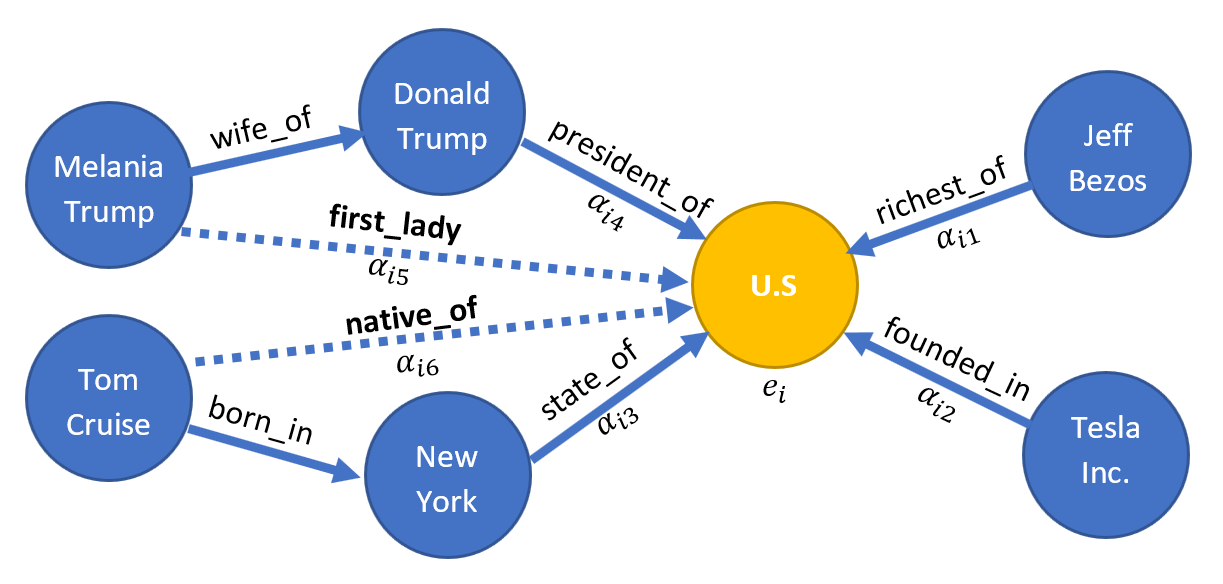
\includegraphics[width=\textwidth,height=\textheight,keepaspectratio]{images/graph_example.png}
\caption{Hình ví dụ 1}
\label{fig:vd1}
\end{figure}

Mỗi chủ thể sẽ bao gồm nhiều đặc trưng khác nhau, ví dụ chiều cao của tổng thống Donald Trump là 1.9. Khi đó ta giả định $f_\text{height}$ là hàm đo chiều cao của một đối tượng, vậy $f_\text{height}(entity_\text{Trump}) = 1.9$, $1.9$ thể hiện độ lớn của độ đo $f_\text{height}$ Tuy nhiên nếu ta áp dụng hàm đó với những chủ thể khác thì không thể đo được hoặc không có giá trị, ví dụ ta muốn tính chiều cao của $\textit{Nước Mỹ}$, hay diện tích của Donald Trump. Vì vậy ta cho giá trị của độ đo đó bằng $0$, $f_\text{height}(entity_\text{U.S}) = 0$, tức độ lớn của đặc trưng chiều cao $\textit{height}$ bằng 0. Đối với những hàm không đo độ lớn mà là hàm đo giá trị thì ta có thể biểu diễn dưới dạng nhiều độ đo đơn vị nhỏ hơn với kết quả của từng độ đo là các xác xuất của từng giá trị khác nhau, ví dụ ta muốn biết đặc trưng \textbf{vợ} của chủ thể là Donal Trump. Ta sẽ biểu diễn bằng cách chia nhỏ hàm đo đó thành các hàm đo nhỏ hơn như sau : \(f_\text{wife}(e_\text{Trump}) = f_\text{wife is Taylor}(e_\text{Trump}); f_\text{wife is Melania}(e_\text{Trump});... \). Với mỗi hàm $f_\text{wife is Melania}$ thể hiện cho độ lớn xác xuất đặc trưng vợ là Melania của chủ thể. Khi đó mỗi chủ thể đều có thể được biểu diễn với nhiều độ đo đơn vị nào đó, hay nói cách khác, mỗi chủ thể $e_i$ đều có thể được biểu diễn bởi một vector $\overrightarrow{e_i}$, với mỗi số trong vector $\overrightarrow{e_i}$ thể hiện cho độ lớn đặc trưng của một độ đo $f_{feature}$ nào đó.  Ví dụ : $\overrightarrow{e_\text{Trump}} = [1.9_{\text{heigh}}, 0_{\text{area}}, 1_\text{wife is Melania}, 0_\text{wife is Taylor}]$, và 
$$
\overrightarrow{e}=\Big[ \bigparallel_{t \in features}^{T} f_{t}{}(e) \Big]
$$

Trong đó vector $\overrightarrow{e}$ là kết quả của quá trình ánh xạ T chiều đặc trưng khác nhau, hay nói cách khác mỗi giá trị trong vector \(\overrightarrow{e}\) là để thể hiện cho độ lớn hoặc xác xuất của các đặc trưng thể hiện giá trị tương ứng của một độ đo đặc trưng $f_t$ nào đó của chủ thể $e_i$. Để thuận tiện trong quá trình tính toán ta đưa các giá trị của các vector để đảm bảo nó luôn nằm trong đoạn $[0, 1]$ bằng cách \textbi{chuẩn hóa} $\overrightarrow{e} = || e ||_p$, với $p$ không nhỏ hơn 1.

Kỹ thuật ánh xạ các chủ thể theo không gian có số chiều thấp đảm bảo thông tin đồ thị với mỗi chiều thể hiện cho một đặc trưng để tạo ra một vector biểu diễn cho một thực thể được gọi là quá trình nhúng (embedding). Để biểu diễn một đồ thị tri thức ta có thể nhúng đồ thị với nhiều cách khác nhau bao gồm : nhúng các thực thể (Node Embedding), nhúng cạnh (Edge Embedding), Nhúng bộ phận cấu trúc (Substructure Embedding), và nhúng toàn bộ đồ thị (Whole-Graph Embedding). Khi ta nhúng Khi đó mỗi thực thể sẽ bao gồm nhiều  lên một độ đo trên tạo ra các thực thể nhúng (entities embedding), tương tự kết quả của quá trình nhúng các quan hệ gọi là (relations embedding).

Ngoài phương pháp á
Ở phần này chúng tôi sẽ giới thiệu tóm lược về mạng đồ thị chú ý (GATs \cite{velivckovic2017graph}) và cải tiến của chúng tôi trên lớp GAT mà chúng tôi gọi là \textit{mạng cộng tác đồ thị chú ý} CGAT, và sau đó chúng tôi áp dụng vào để xây dựng đồ thị theo mô hình KGAT \cite{nathani2019learning} để tối ưu quá trình dự đoán các mối quan hệ. 

\subsection{Mô hình GAT}

Mạng đồ thị tích chập (Graph Convolutional Networks \citetitle{schlichtkrull2018modeling}{GCNs}) giúp tổng hợp thông tin bằng cách tính trung bình thông tin từ các thực thể lân cận, tuy nhiên cách này sẽ làm cho các thực thể có trọng số ngang bằng nhau không biểu diễn đúng thông tin trong thế giới thực. Để giải quyết vấn đề đó, GATs \cite{velivckovic2017graph} ra đời để đối xử với các thực thể lân cận bằng sự quan trọng của chúng.

Đầu vào của mô hình là vector biểu diễn đặc trưng của từng thực thể (entity) $E = \Big\{\overrightarrow{e_1}, \overrightarrow{e_2}, ...,  \overrightarrow{e_N}\Big\}$. Và mục tiêu của chúng ta là biến đổi thành một đặc trưng đầu ra mới $E'' = \Big\{\overrightarrow{e''_1}, \overrightarrow{e''_2}, ...,  \overrightarrow{e''_N}\Big\}$; với $\overrightarrow{e_i}$ và $\overrightarrow{e''_i} \in \mathbb{R}^T$ tương ứng là vector nhúng đầu vào và vector đầu ra của của thực thể $e_i$, N là số lượng của các thực thể, T là số miền nhúng đặc trưng đầu vào.

Mô hình sẽ đi qua hai quá trình biến đổi vector đặc trưng $\overrightarrow{e_i}$ và có thể tóm lược như sau :
\begin{align}
\overrightarrow{e_i} \longrightarrow \overrightarrow{e'_i} \longrightarrow \overrightarrow{e''_i}
\end{align}

Ở quá trình biên đổi đầu tiên, mô hình sẽ tổng hợp thông tin từ các thực thể lân cận và ghép chồng lên nhau để tạo ra vector $\overrightarrow{e'_i}$ sau đó mô hình sẽ dùng vector $\overrightarrow{e'_i}$ để coi là vector nhúng của thực thể cho lớp mới và tiếp tục quá trình tổng hợp từ các thông tin lân cận và tạo ra vector $\overrightarrow{e''_i}$ cuối cùng.

Đầu tiên để tham số hóa quá trình biến đổi tuyến tính, ta cần một trọng số $W \in \mathbb{R}^{N_e \times T}$ ánh xạ vector đầu vào thành một vector mới với miền không gian lớn hơn và một hàm chú ý $a$ chúng ta tùy chọn :

\begin{align}
\centering
{e_{ij}}&={a(W \overrightarrow{e_i}, W \overrightarrow{e_j})}
\end{align}

trong đó $e_{ij}$ là giá trị chú ý của một cạnh $(e_i, e_j)$ trong đồ thị $\mathcal{G}$ hay $e_{ij}$ thể hiện sự quan trọng của đặc trưng cạnh $(e_i, e_j)$ so với thực thể $e_i$. Sau đó, chúng ta áp dụng hàm \textit{softmax} qua tất cả các giá trị nhúng của hàng xóm để tạo ra $\alpha_{ij}$ . Quá trình tổng hợp các sự chú ý được thể hiện ở biểu thức sau : 

\begin{align}
\centering
{\overrightarrow{a_{ij}}}&={\sigma\left(\sum_{j\in \mathcal{N}_i} {\alpha_{ij} \mathbf{W} \overrightarrow{e_j} }\right)}
\end{align}

Tiếp theo mô hình GAT sẽ đi qua \textit{lớp chú ý đa đỉnh}(multi-head attention) để ổn định quá trình học bằng cách ghép $A$ đỉnh chú ý với nhau :

\begin{align}
{\overrightarrow{x'_i}}&={\bigparallel_{a=1}^{A}\sigma\left(\sum_{j\in \mathcal{N}_i}\alpha_{ij}^{a} \mathbf{W}^{a} \overrightarrow{x_{j}} \right)}
\end{align}

trong đó phép $||$ biểu diễn quá trình ghép chồng lên nhau và $\sigma$ là bất kỳ hàm biến đổi phi tuyến tính nào, $\alpha_{ij}^a$ là hệ số chú ý được chuẩn hóa của cạnh $(e_i, e_j)$ được tính từ lớp thứ $a^{th}$	 cơ chế chú ý. Cuối cùng $\overrightarrow{x'_i}$ được coi là vector thực thể nhúng mới và cho vào lớp chú ý đa đỉnh với đầu ra thay vì ghép chồng như trên thì được tính trung bình như công thức sau :

\begin{align}
{\overrightarrow{x''_i}}&={\sigma\left(\frac{1}{A} \sum_{a=1}^{A}\sum_{j\in \mathcal{N}_i}\alpha_{ij}^{a} \mathbf{W}^{a} \overrightarrow{x'_{j}} \right)}
\end{align}

\subsection{Knowledge Base Attention Network (KBAT)}

Trong phần này sẽ trình bày về mô hình Knowledge Base Attention (KBAT \cite{nathani2019learning}), là một mô hình cải tiến dựa trên mô hình GAT ở trên bằng cách lấy thêm thông tin của mối quan hệ trên một cạnh. Mục tiêu của mô hình là tạo ra hai ma trận mới biểu thị cho \textbf{ma trận nhúng thực thể} và \textbf{ma trận nhúng quan hệ}. Mô hình sẽ biến đổi từ ma trận thực thể $\mathbf{E} \in \mathbb{R}^{N_e \times T}$ và ma trận quan hệ $\mathbf{R} \in \mathbb{R}^{N_r \times P}$ để tạo thành một ma trận thực thể mới $\mathbf{E'} \in \mathbb{R}^{N_e \times T'}$ và ma trận quan hệ mới $\mathbf{R'} \in \mathbb{R}^{N_r \times P'}$, trong đó với mỗi dòng thứ $i^{\text{th}}$ trong ma trận với trọng số tương ứng biểu thị cho một thực thể $e_i$ hoặc một mối quan hệ $r_i$; $N_e$ hoặc $N_r$ tương ứng là số lượng của tập thực thể và tập quan hệ; trong khi $T$ và $P$ tương ứng là số chiều đầu vào của vector nhúng; thì $T'$ và $P'$ tương ứng là số chiều của vector nhúng đầu ra. Các ma trận trọng số trên được khởi tạo ngẫu nhiên theo phân phối chuẩn hoặc tái huấn luyện(pre-train) bằng mô hình TransE \cite{bordes2013translating} .

Trong đồ thị, mỗi cạnh của thực thể không chỉ được biểu diễn thông tin bởi thực thể đầu $e_\text{head}$ và thực thể đích $e_\text{tail}$ mà có các quan hệ giữa chúng. Hơn nữa trong một cạnh, các thực thể còn có thể đóng nhiều vai trò khác nhau phụ thuộc vào các loại quan hệ khác nhau. Vì vậy phương pháp KBGAT bổ sung thêm thông tin của một vector nhúng quan hệ vào một cạnh  nhúng $(\overrightarrow{e_\text{i}}, \overrightarrow{r_k}, \overrightarrow{e_\text{j}})$. Tuy nhiên một vector $\overrightarrow{e_i}$ hay $\overrightarrow{r_k}$ không thể biểu thị một cách đầy đủ tri thức của một thực thể $e_i$ hay quan hệ $r_k$ trong một đồ thị, vì một tri thức sẽ có thể có mối liên hệ với những tri thức lân cận hay nói cách khác một \textbf{thực thể nhúng} (entity embedding) hay một \textbf{quan hệ nhúng} (relation embedding) sẽ cần thêm thông tin của các vector nhúng của thực thể lân cận và quan hệ lân cận khác để có thể là một đại diện đầy đủ . Chính vì vậy phương pháp \textit{n-hop neighborhood} \cite{lin2018multi} sẽ giúp bổ sung thêm thông tin lân cận của thực thể $e_i$ và quan hệ $r_k$ bằng cách ghép chồng để tạo thành một vector mới theo công thức sau :
\begin{align}
{\overrightarrow{h_i} = [\overrightarrow{e_i} \bigparallel_{\text{axis}=1} \overrightarrow{e_{i_{\text{n-hop}}}}]} \hspace{0.5cm};\hspace{1.5cm}&
{\overrightarrow{g_k} = [\overrightarrow{r_k} \bigparallel_{\text{axis}=1} \overrightarrow{r_{k_{\text{n-hop}}}}]}
\end{align}

Trong đó $\overrightarrow{h_i}$, $\overrightarrow{g_k}$ tương ứng là vector nhúng mới của thực thể $e_i$ và các thực thể lân cận ($e_{i_{\text{n-hop}}}$) hay quan hệ $r_k$ và các quan hệ lân cận ($r_{k_{\text{n-hop}}}$); ký hiệu $\bigparallel_{\text{axis}=1}$ biểu thị cho phép xếp chồng lên nhau. Các vector $\overrightarrow{e_{i_{\text{n-hop}}}}$ và $\overrightarrow{r_{k_{\text{n-hop}}}}$ được tính bằng tổng vector nhúng của các thực thể hoặc các quan hệ lân cận đi qua $n-hop$ độ sâu bắt đầu từ $e_i$ theo công thức sau : 

\begin{align}
{\overrightarrow{e_{i_{\text{n-hop}}}} = \bigparallel_{d=1}^{\text{n-hop}} \sum_{n \in \mathcal{N}_i} \overrightarrow{e_n^d}} \hspace{0.5cm};\hspace{1.5cm}&
{\overrightarrow{r_{k_{\text{n-hop}}}} = \bigparallel_{d=1}^{\text{n-hop}} \sum_{m \in \mathcal{N}_k} \overrightarrow{r_m^d}}
\end{align}

Với mối thực thể $e_n$ hay quan hệ $r_m$ có độ sâu d (depth) bắt đầu từ thực thể $e_i$, ta sẽ tính tổng các vector nhúng và ghép chồng với nhau.

Để biểu thị cho quá trình biến tuyến tính của vector nhúng, ta cho mỗi vector nhúng đi qua một ma trận trọng số : $\overrightarrow{h'_i} = \mathbf{W}_{\text{entity}} \overrightarrow{h_i}$ 
và $\overrightarrow{g'_i} = \mathbf{W}_{\text{relation}} \overrightarrow{g_i}$. Tuy nhiên để thu được một trọng số mới biểu diễn bộ ba $t^k_{ij} = (e_{\text{head}}, relation, e_{\text{tail}})$ tương ứng với một cạnh trong trong KB. Ta thực hiện quá trình biến đổi tuyến tính đó bằng cách ghép cả thực thể và mối quan hệ với nhau rồi nhân với một ma trận trọng số chung như công thức sau :

\begin{align}
\overrightarrow{t_{ijk}} = \mathbf{W_1} [\overrightarrow{h_i} || \overrightarrow{h_j} || \overrightarrow{g_k}]
\end{align}

trong đó $\overrightarrow{t_{ijk}}$ là một vector nhúng biểu diễn cho một bộ ba $t^k_{ij}$. Các vector $\overrightarrow{h_i}$, $\overrightarrow{h_j}$ và $\overrightarrow{g_j}$ tương ứng là vector nhúng của các thực thể $e_i$, $e_j$ và quan hệ $r_k$. $\mathbf{W_1} \in \mathbb{R}^{3 T \times S^\text{batch}}$ . Để áp dụng cơ chế chú ý (attention mechanisms \cite{vaswani2017attention}), ta cần học sự quan trọng của một cạnh $t_{ij}^k$ bởi giá trị của $b_{ij}^k$. Để tham số hóa quá trình biến đổi tuyến tính ta nhân với ma trận trọng số $\mathbb{W}_{2}$ và lấy giá trị chú ý tuyệt đối bằng hàm $LeakyRelu$ theo công thức sau :

\begin{align}
b_{ijk} = \text{LeakyRelu}\Big( \mathbf{W_2} t_{ijk} \Big)
\end{align}

Sau đó, với mỗi độ lớn của $b^k_{ij}$ được cho qua hàm \textit{softmax} để tính giá trị thể hiện xác xuất của từng giá trị chú ý $\alpha_{ijk}$ đối với từng bộ ba .

\begin{align}
{\alpha_{ijk}}&={\text{softmax}_{jk}(b_{ijk})} =\frac{\text{exp}(b_{ijk})}{\sum_{n\in \mathcal{N}_i} \sum_{r\in \mathcal{R}_{in}}\text{exp}(b_{inr})}
\end{align}

trong đó $\mathcal{N}_i$ là tập hợp những thực thể kế cận của $e_i$; $\mathcal{R}$ tập hợp những quan hệ nối hai thực thể $e_i$ và $e_j$. Để tăng cường đặc trưng cạnh tương ứng với từng xác xuất, ta sẽ nhân giá trị chú ý tương đối $\alpha_{ijk}$ với vector nhúng $\overrightarrow{t_{ijk}}$ đã được biến đổi tuyến tính ban đầu . Tương tự như GAT, mô hình sẽ tạo ra vector thực thể nhúng mới với đã được tổng hợp từ các thực thể lân cận .

\begin{align}
{\overrightarrow{h'_{i}}}&={\sigma\left(\sum_{j \in \mathcal{N}_i} \sum_{k \in \mathcal{R}_{ij}} \alpha_{ijk} \overrightarrow{t_{ijk}}\right)}
\end{align}

Tương tự như mạng đồ thị chú ý ở trên, mô hình sẽ đi qua lớp chú ý đa đỉnh để ổn định quá trình học bằng cách ghép A đỉnh chú ý với nhau theo công thức sau :

\begin{align}
\overrightarrow{h'}_i=\bigparallel_{m=1}^{M} \sigma\left(\sum_{j\in \mathcal{N}(i)}\alpha_{ijk}^{m}t^{m}_{ijk}\right)
\end{align}

Như quá trình biến đổi tuyến tính của ma trận mối quan hệ ở trên, ma trận $R$ đầu vào sẽ được nhân với một vector nhúng $W$ quan hệ để tạo ra một ma trận mới biểu thể tập hợp các quan hệ nhúng mới :

\begin{align}
R' = R \mathbf{W^R}; \hspace{2cm} \text{Trong đó : } \mathbf{W^R} \in \mathbb{R}^{P \times P'}
\end{align}

Trong đó $\mathbf{W^R}$ là ma trận trọng số thể hiện quá trình biến đổi tuyến tính,$P$ và $P'$ lần lượt là số chiều của vector quan hệ nhúng đầu vào và đầu ra. Và trong trường hợp này  $P'$ phải bằng số chiều của vector nhúng thực thể.

Đến đây, ta đã có hai ma trận $H'$ và $R'$ tương ứng là ma trận quan hệ và ma trận thực thể. Mô hình sẽ đi qua lớp cuối chú ý cùng bằng cách tiếp tục đi qua lớp mạng đồ thị chú ý tương tự ở trên nhưng thay vì ghép chồng thì ta thực hiện tính trung bình theo công thức sau :

\begin{align}
{\overrightarrow{h''_{i}}}&={\sigma\left(\frac{1}{M} \sum_{m=1}^{M} \sum_{j \in \mathcal{N}_i} \sum_{k \in \mathcal{R}_{ij}} \alpha'^m_{ijk} t'^m_{ijk}\right)}
\end{align}

Tương tự như trên, nhưng $\alpha'^m_{ijk}$ và $t'^m_{ijk}$ tương ứng là các vector được nhúng trên các mối quan hệ và thực thể mới.

Sau quá trình nhúng trên, ta sẽ có một ma trận thực thể $H''$ và quan hệ $R''$ mới đã được tổng hợp thêm một lần nữa. Tuy nhiên ta muốn biểu diễn ma trận thực thể với số chiều mới, ta thực hiện phép biến đổi sau :


\begin{align}
\mathbf{E'} = \mathbf{W}^E \mathbf{E}^t + \mathbf{H''}
\end{align}

Trước và sau mỗi lớp mạng đồ thị chú ý chúng tôi đề thực hiện chuẩn hóa.


Sau quá trình trên chúng ta đã tạo ra được ma trận nhúng thực thể và quan hệ. 

Our model borrows the idea of a translational
scoring function from (Bordes et al., 2013), which
learns embeddings such that for a given valid triple $t^k_{ij} = (e_i, r_k, e_j)$, the condition $\vec{h_i}+\vec{g_k} \approx \vec{h_j}$ holds, i.e., $e_j$ is the nearest neighbor of $e_i$ connected via relation $r_k$.

 Specifically, we try to learn entity and relation embeddings to minimize the L1-norm dissimilarity measure given by $d_{t_{ij}} = \big|\big|\vec{h_i}+ \vec{g_k}-\vec{h_j}\big|\big|_1$.

We train our model using hinge-loss which is
given by the following expression


\begin{align}
{L(\Omega)}&={\sum_{t_{ij} \in S} \sum_{t'_{ij} \in S'} \text{max}\{d_{t'_{ij}} - d_{t_{ij}} + \gamma , 0 \}}
\end{align}

where $\gamma > 0$ is a margin hyper-parameter, $S$ is the set of valid triples, and $S'$ denotes the set of invalid
triples, given formally as

\begin{align}
{S'}&={\underbrace{\{ t^k_{i'j} | e'_i \in \mathcal{E}\setminus e_i\}}_{\text{thay thế thực thể đầu}}\cup \underbrace{\{ t^k_{ij'} | e'_j \in \mathcal{E}\setminus e_j\}}_{\text{thay thế thực thể đuôi}}}
\end{align}

where $\omega^m$ represents the $m-th$ convolutional filter,
\(\omega\) is a hyper-parameter denoting number of filters
used, \(\ast\) is a convolution operator, and \(\mathbf{W} \in \mathbb{R}^{\Omega k \times 1}\)
represents a linear transformation matrix used to
compute the final score of the triple. The model is
trained using soft-margin loss as

\begin{align}
\mathcal{L} = \sum_{t^k_{ij} \in \{S \cup S'\}} \text{log}(1 + exp(l_{t^k_{ij}} . f(t^k_{ij}))) + \frac{\lambda}{2} \parallel{\mathbf{W}}\parallel_2^2
\end{align}

where $l_{t^k_{ij}} = \begin{cases}
1 &\text{for } t^k_{ij} \in S \\
-1 &\text{for } t^k_{ij} \in S' \\
\end{cases}$

Attention 

CAttention \cite{cordonnier2020multi}

ConvKB \cite{nguyen2017novel}

